%--------------------------------Dependencies----------------------------------%
%   tikz                                                                       %
%-------------------------------Main Document----------------------------------%
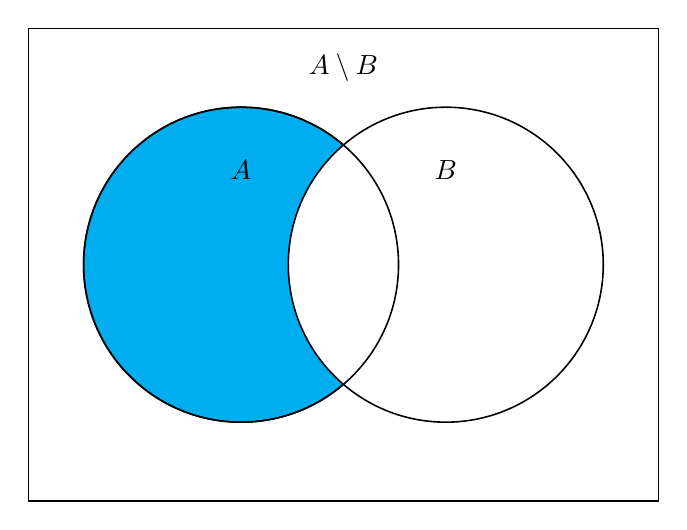
\begin{tikzpicture}[line width=0.2mm]

    % Coordinates for the centers of the circles.
    \coordinate (C1) at (-1.3, 0);
    \coordinate (C2) at ( 1.3, 0);

    % Coordinates for the labels.
    \coordinate (A) at (-1.3, 1.2);
    \coordinate (B) at ( 1.3, 1.2);
    \coordinate (U) at ( 0.0, 2.5);

    % Rectangle indicating the universe set.
    \draw (-4, -3) rectangle (4, 3);

    % Draw the two circles.
    \draw[fill=cyan]              (C1) circle (2);
    \draw[fill=white, draw=black] (C2) circle (2);

    % Add an outline to the left circle.
    \draw (C1) circle (2);

    % Labels.
    \node at (A) {$A$};
    \node at (B) {$B$};
    \node at (U) {$A\setminus{B}$};
\end{tikzpicture}